\newpage
\subsection{Оперативное планирование продаж}
\label{bp:salesplan}


Оперативным планированием продаж на ПРЕДПРИЯТИИ занимаются менеджеры отдела продаж ООО ТД ''ФОРМАТ''. Все заказы/заявки оформляются ими в системе 1С: УПП (рис. \ref{pic:Рабочее место менеджера.jpg}).

Заявки/заказы от покупателей каждому менеджеру поступают по электронной почте, через мессенджеры. Форма подачи свободная (рис. \ref{pic:I.2.}).

После получения заявки менеджер в 1С: УПП производит следующие действия:
\begin{itemize}
    \item проверяет наличие ранее разработанных активных технологических карт по ГП через вкладку ''Технологические карты'' (рис. \ref{pic:II.4.jpg}); 
    \item проверяет, через отчет ''Загрузка оборудования по предварительным заявкам'' (рис. \ref{pic:I.5.2...jpg}) возможность размещения заказа на производство на ту или иную линию на желаемую дату;
    \item создает документ ''Предварительная заявка'' (рис. \ref{pic:I.5.jpg}) на резервирование времени работы требуемого для изготовления заказа оборудования;
    \item в табличной части указывает номенклатуру ГП, необходимое количество и дату реализации ГП;
    \item после проведения документа автоматически создается ''Заказ на производство'' (рис. \ref{pic:I.5.4.jpg}), в котором дата отгрузки (информация для производства) будет смещена на один день раньше, установленной менеджером;
    \item на основании документа ''Заказ покупателя''
    % \footnote[1]{''Заказ покупателя'' - необходим для формирования заявки на отгрузку, и создания документов ''План отгрузок'' и ''План реализации''.} 
    создает документ ''Заявку на отгрузку'' (рис. \ref{pic:I.5.5.jpg}), в котором указывает дату отгрузки, адрес доставки, номенклатуру ГП, цену реализации, количество единиц ГП. 
    Документ ''Заказ покупателя'' необходим для формирования заявки на отгрузку и создания документов ''План отгрузок'' и ''План реализации''.
   
\end{itemize}


Каждый менеджер после оформления предварительной заявки и создания заказа на производство, сообщает об этом в отдел планирования по электронной почте. %(рис. \ref{pic:VII 1.jpg}). 


 
%При появлении от клиентов заявок от покупателей менеджеры регистрируют в системе СБИС документ ''Заявка покупателя'' (рис. \ref{pic:dd9}). Менеджеры формируют при необходимости счет на оплату из формы документа \ref{pic:dd8} или создают документ «Счет». 

%В системе СБИС менеджеры регистрируют все заявки покупателя.

%Выделено несколько крупных покупателей, по которым до 25 числа каждого месяца требуется создавать заявки покупателей в 1С: УПП. Таких клиентов только 50\%. 
%Составление списка заявок покупателей в системе СБИС 
% на начало месяца 
% можно условно назвать 
% является 
%оперативным планирование продаж.
%
%

\begin{figure}
\begin{center}
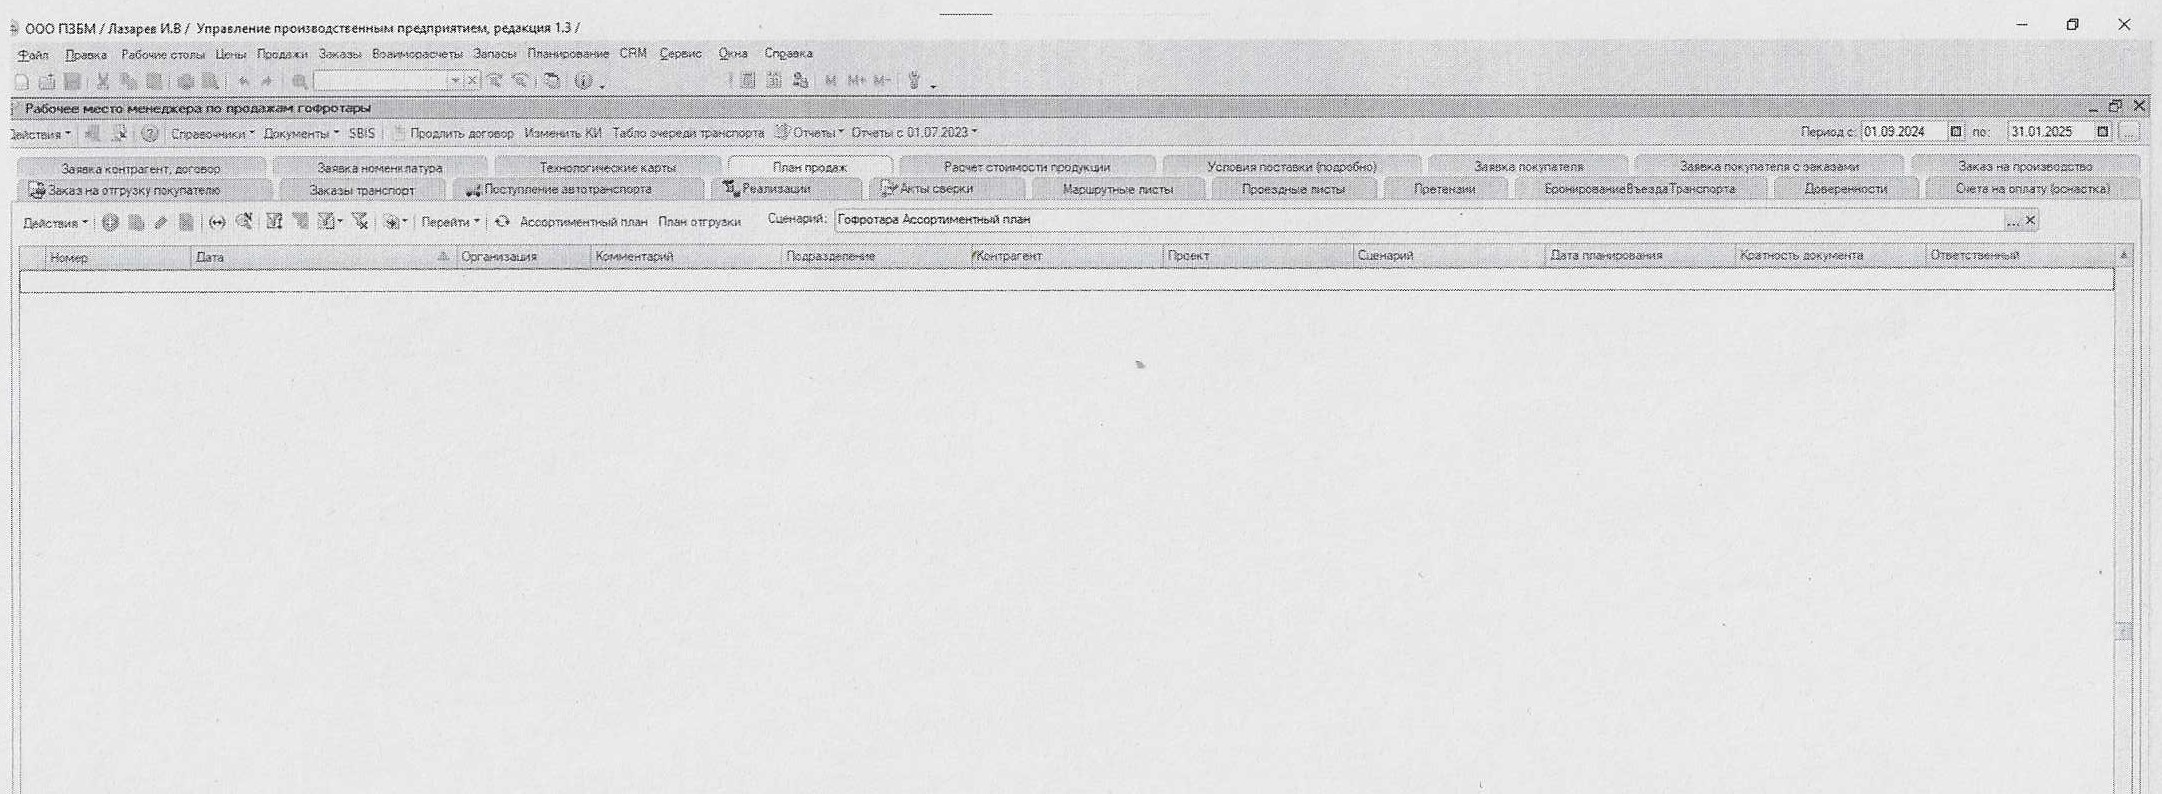
\includegraphics[height=0.25\textheight, angle=90, keepaspectratio]{Pics/Рабочее место менеджера.jpg}
\end{center}
\caption{Рабочий стол менеджера отдела продаж в 1С: УПП}
\label{pic:Рабочее место менеджера.jpg}
\end{figure}
\clearpage

%
\begin{figure}
\begin{center}
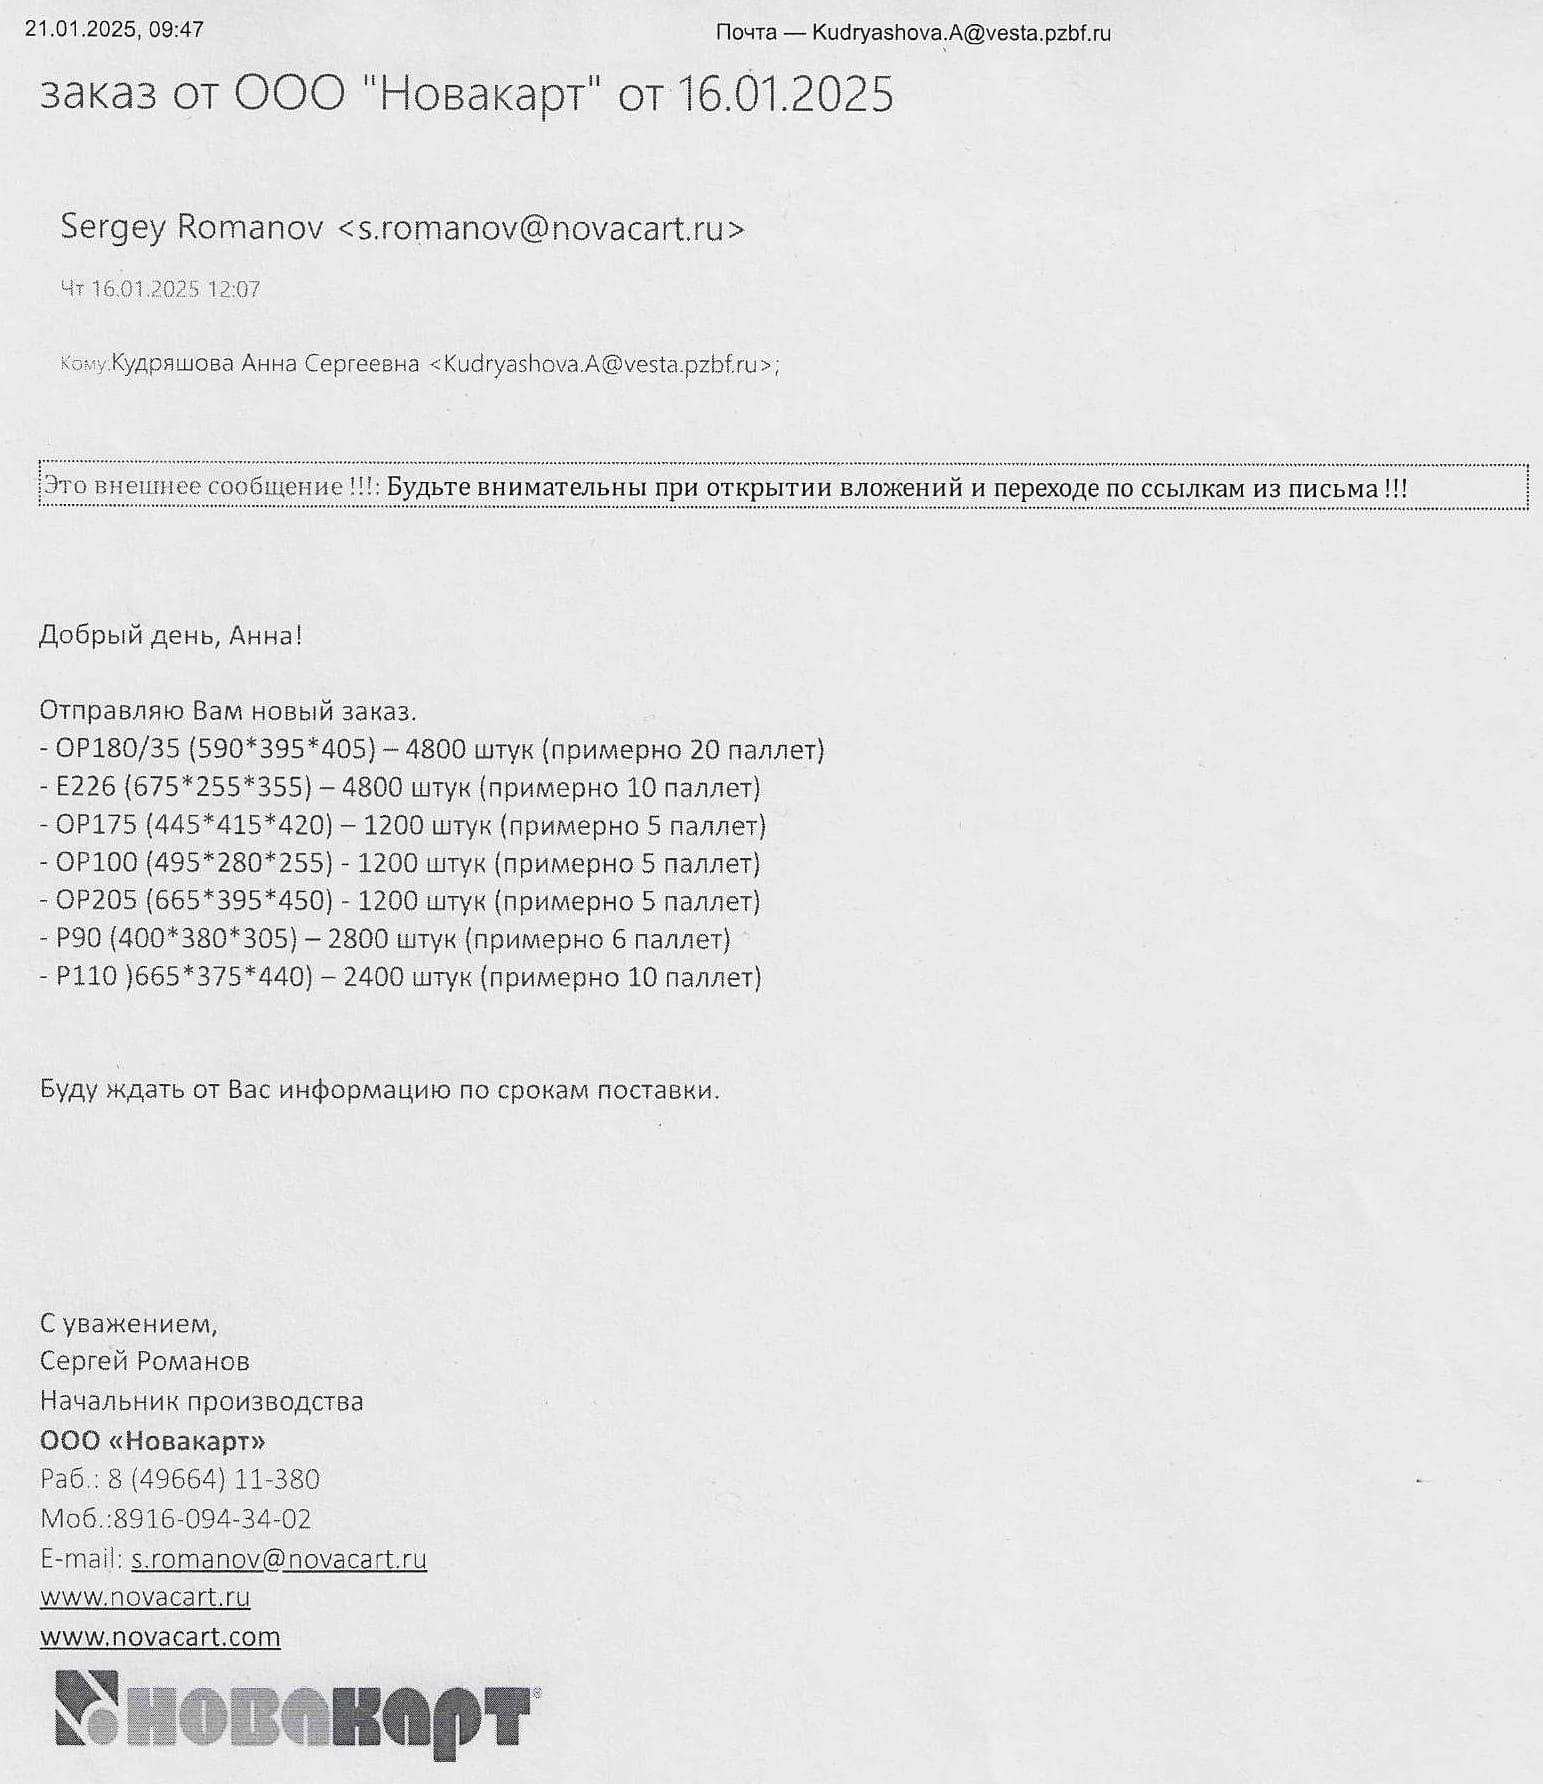
\includegraphics[height=0.7\textheight, keepaspectratio]{Pics/I.2..jpg}
\end{center}
\caption{Вид заявки от покупателя}
\label{pic:I.2.}
\end{figure}
\clearpage


\begin{figure}
\begin{center}
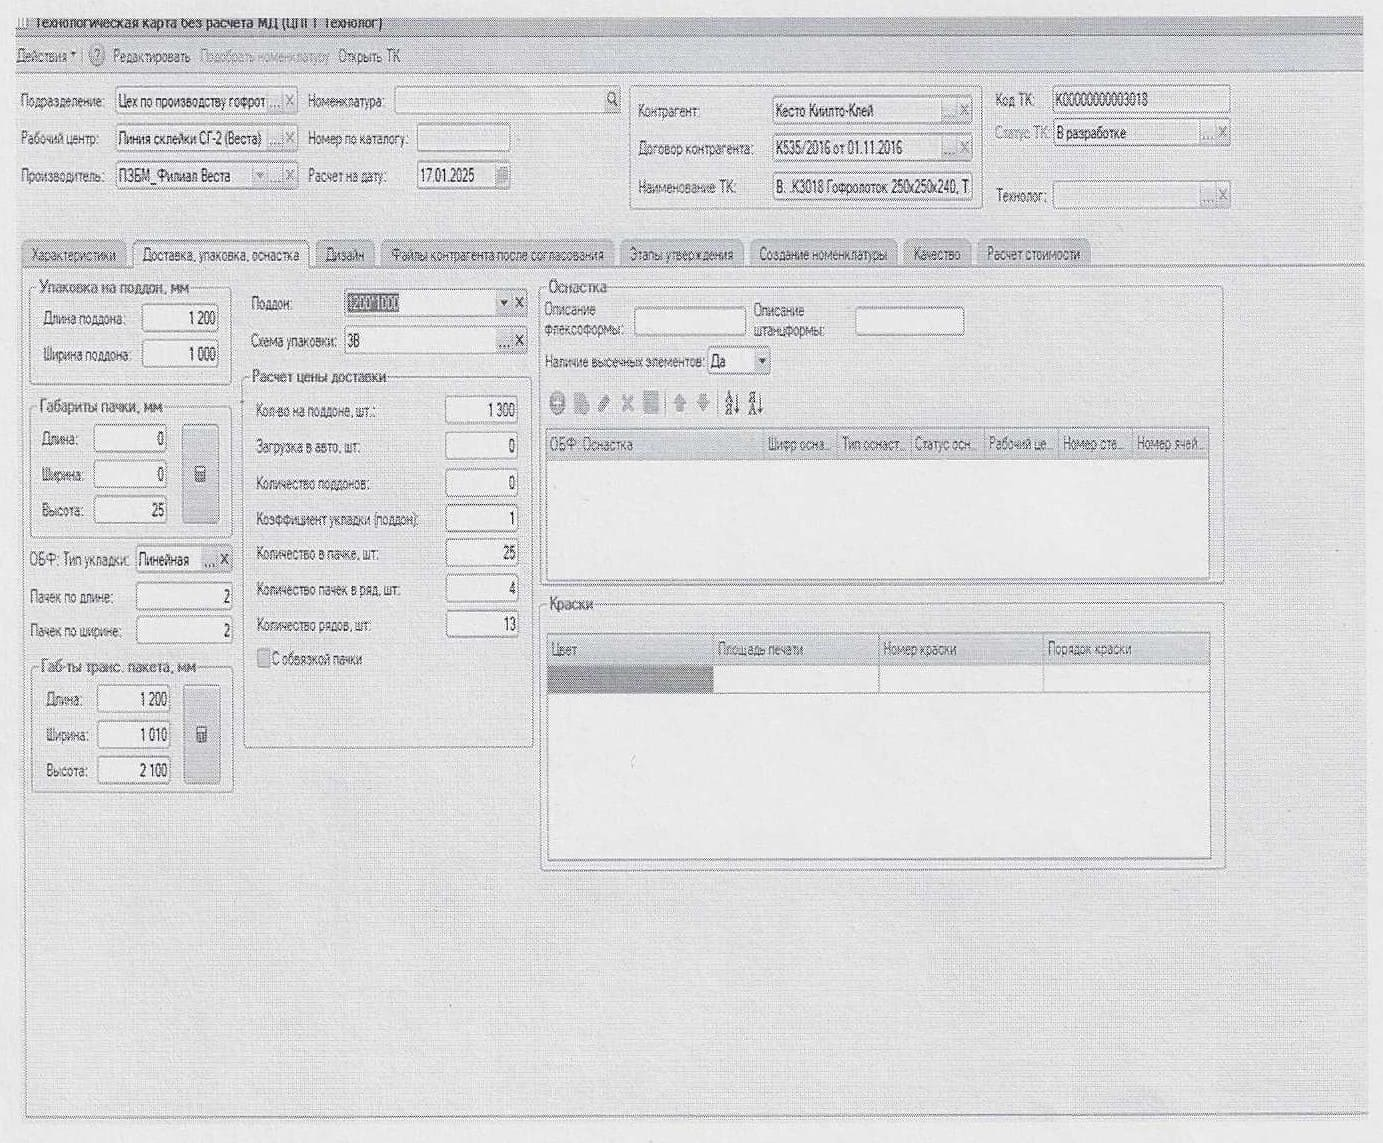
\includegraphics[height=0.5\textheight,  keepaspectratio]{Pics/II.4.jpg}
\end{center}
\caption{Форма Технологическая карта}
\label{pic:II.4.jpg}
\end{figure}
\clearpage



\begin{figure}
\begin{center}
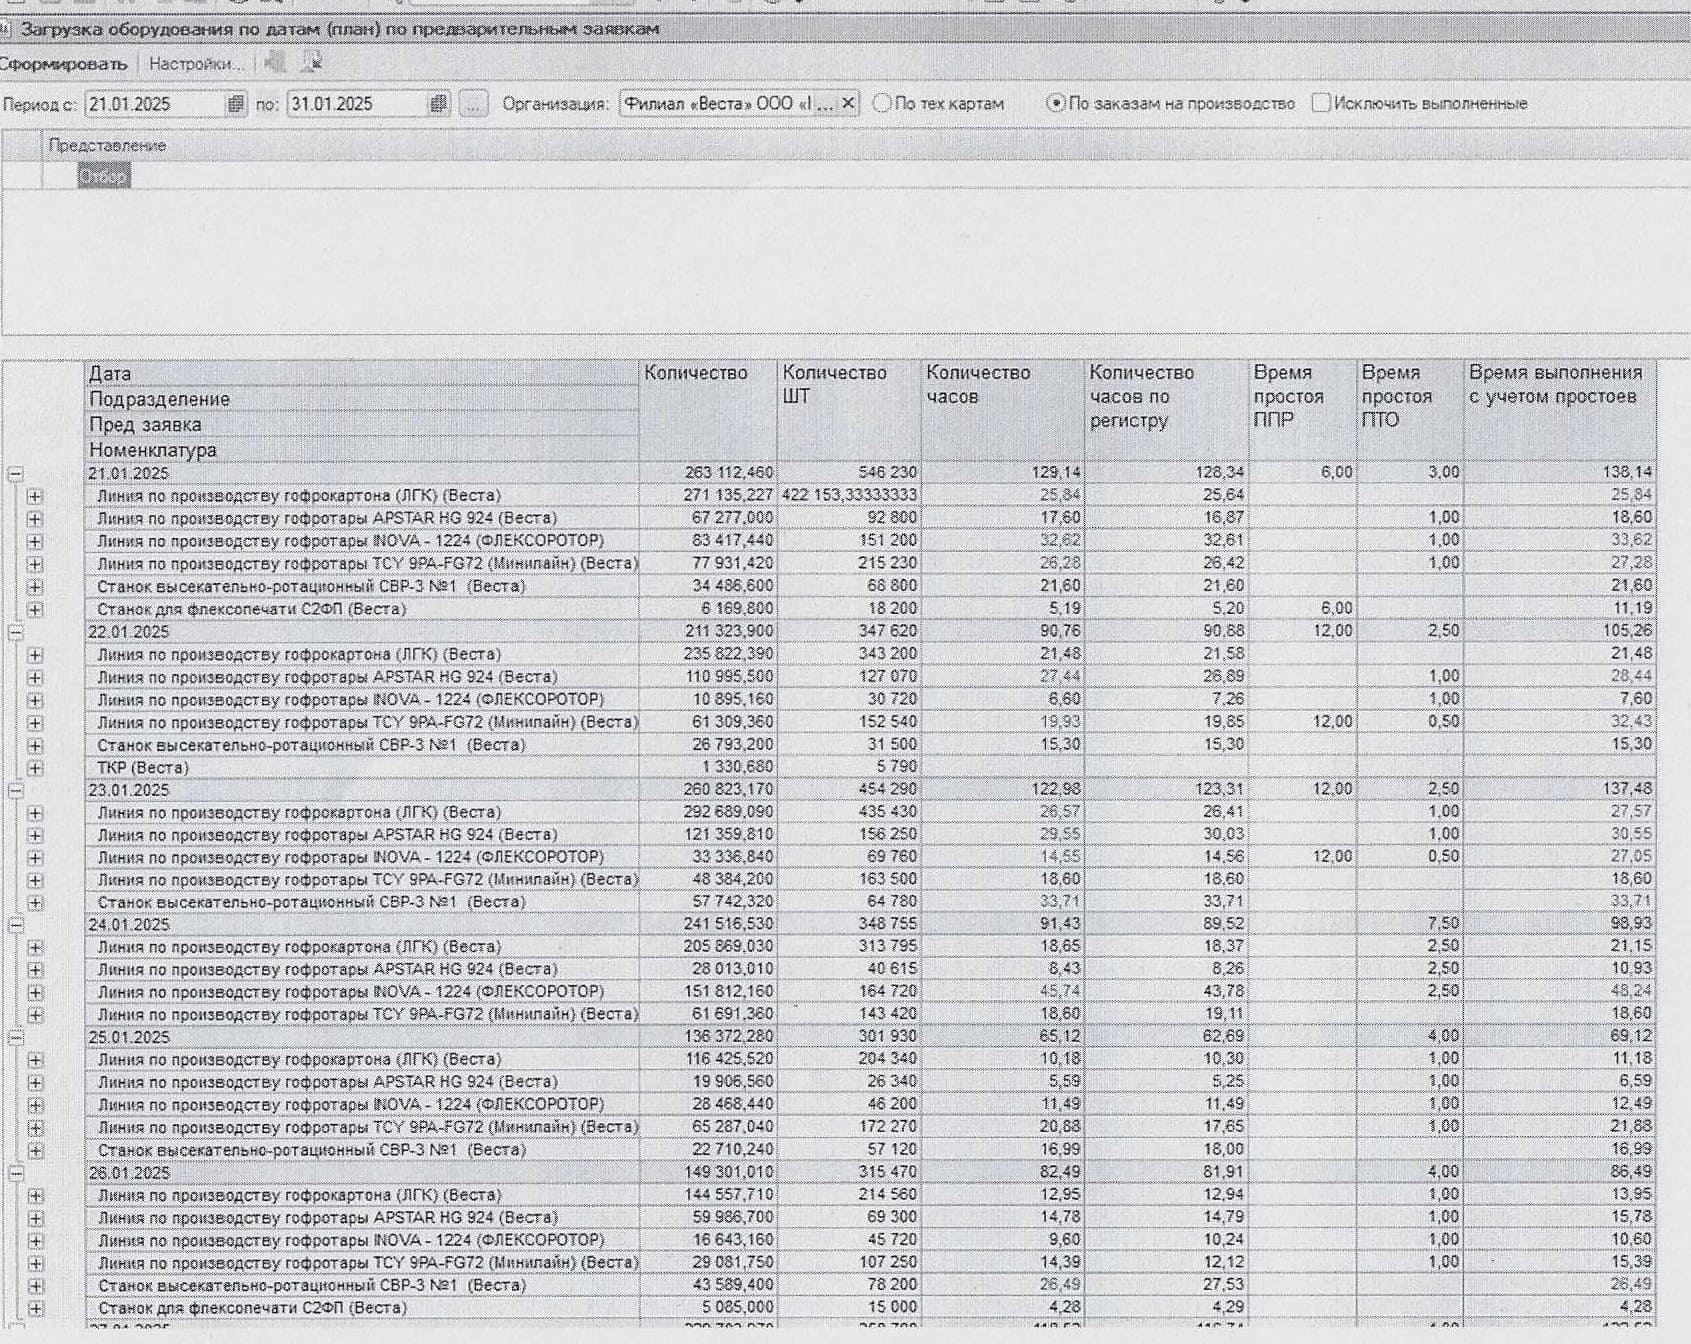
\includegraphics[height=0.5\textheight, keepaspectratio]{Pics/I.5.2...jpg}
\end{center}
\caption{Форма отчета Загрузка оборудования по предварительным заявкам}
\label{pic:I.5.2...jpg}
\end{figure}
%\clearpage



\begin{figure}
\begin{center}
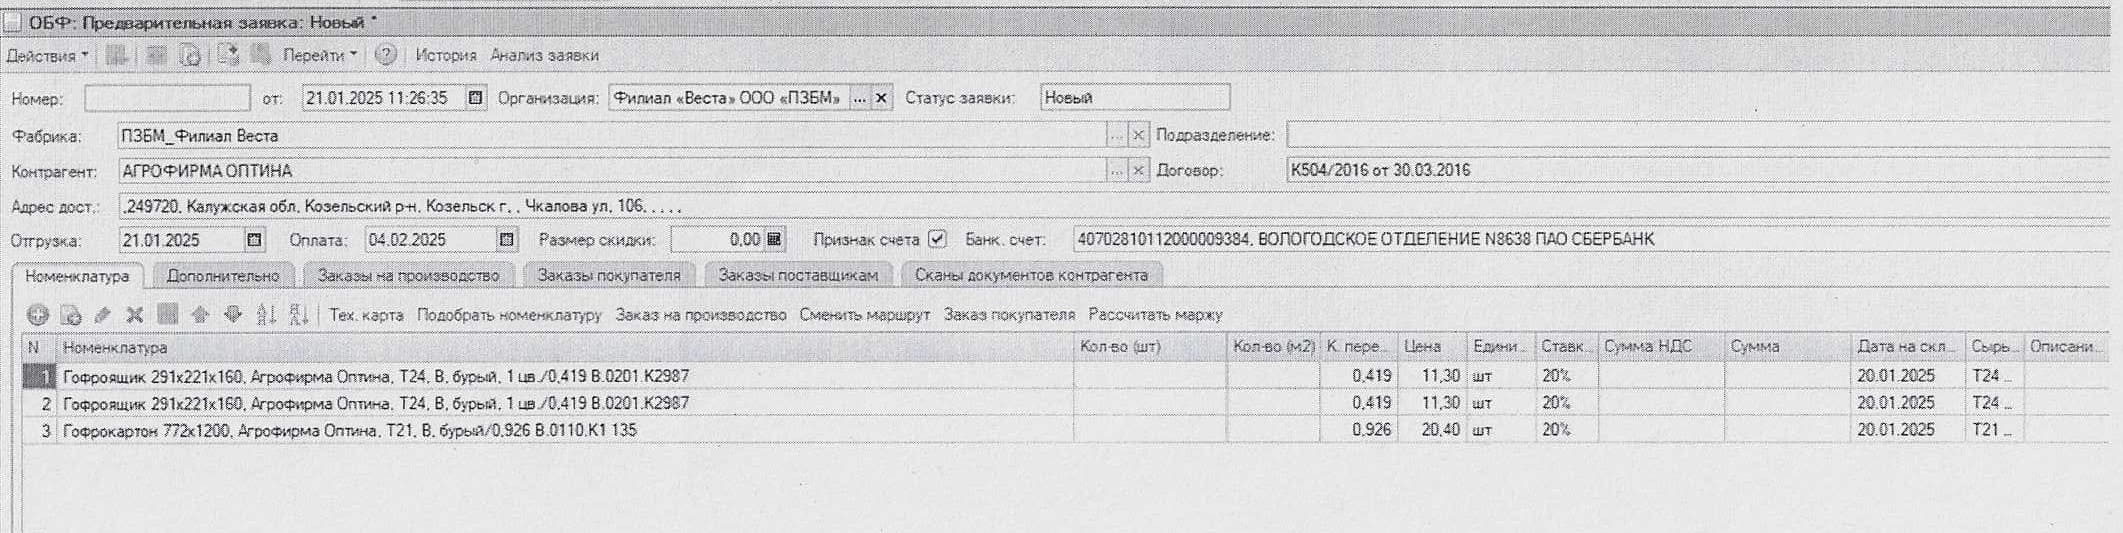
\includegraphics[height=0.15\textheight,  keepaspectratio]{Pics/I.5.jpg}
\end{center}
\caption{Форма создания предварительной заявки}
\label{pic:I.5.jpg}
\end{figure}
\clearpage

\begin{figure}
\begin{center}
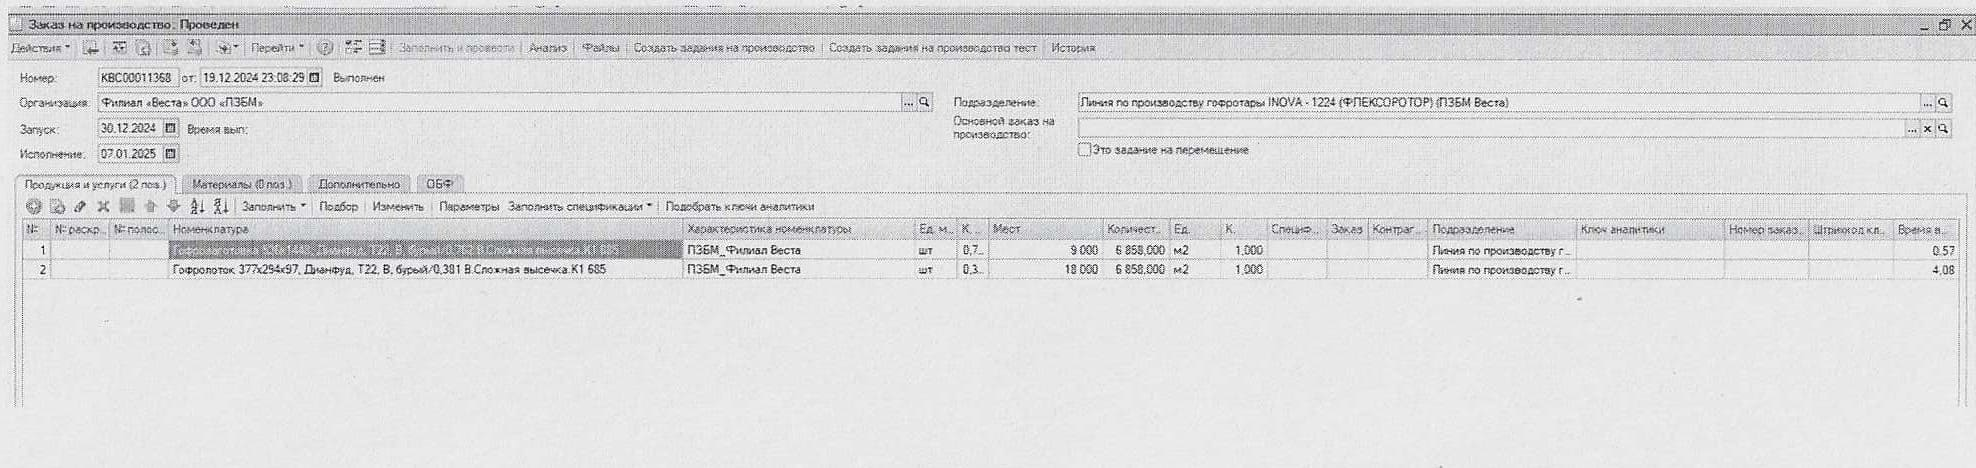
\includegraphics[height=0.15\textheight,  keepaspectratio]{Pics/I.5.4.jpg}
\end{center}
\caption{Форма заказ на производство}
\label{pic:I.5.4.jpg}
\end{figure}
%\clearpage

\begin{figure}
\begin{center}
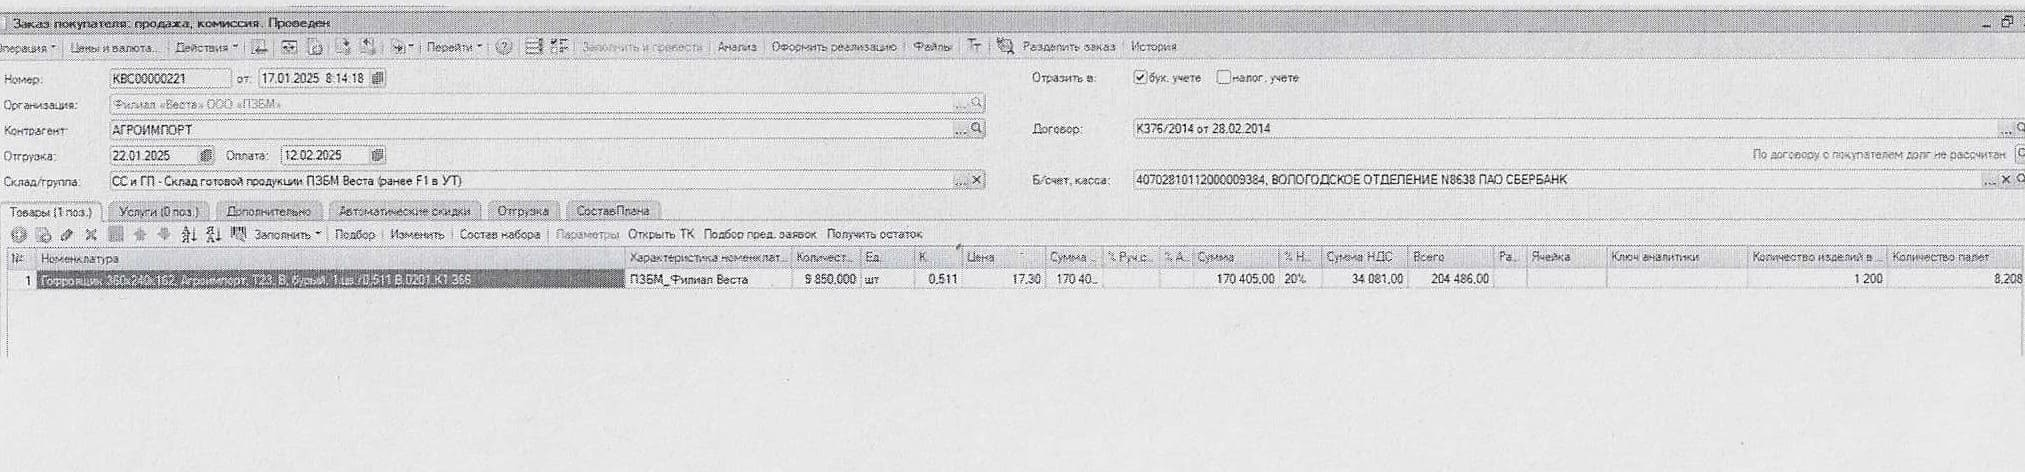
\includegraphics[height=0.15\textheight, keepaspectratio]{Pics/I.5.5.jpg}
\end{center}
\caption{Форма заявка покупателя}
\label{pic:I.5.5.jpg}
\end{figure}
\clearpage

%\begin{figure}
%\begin{center}
%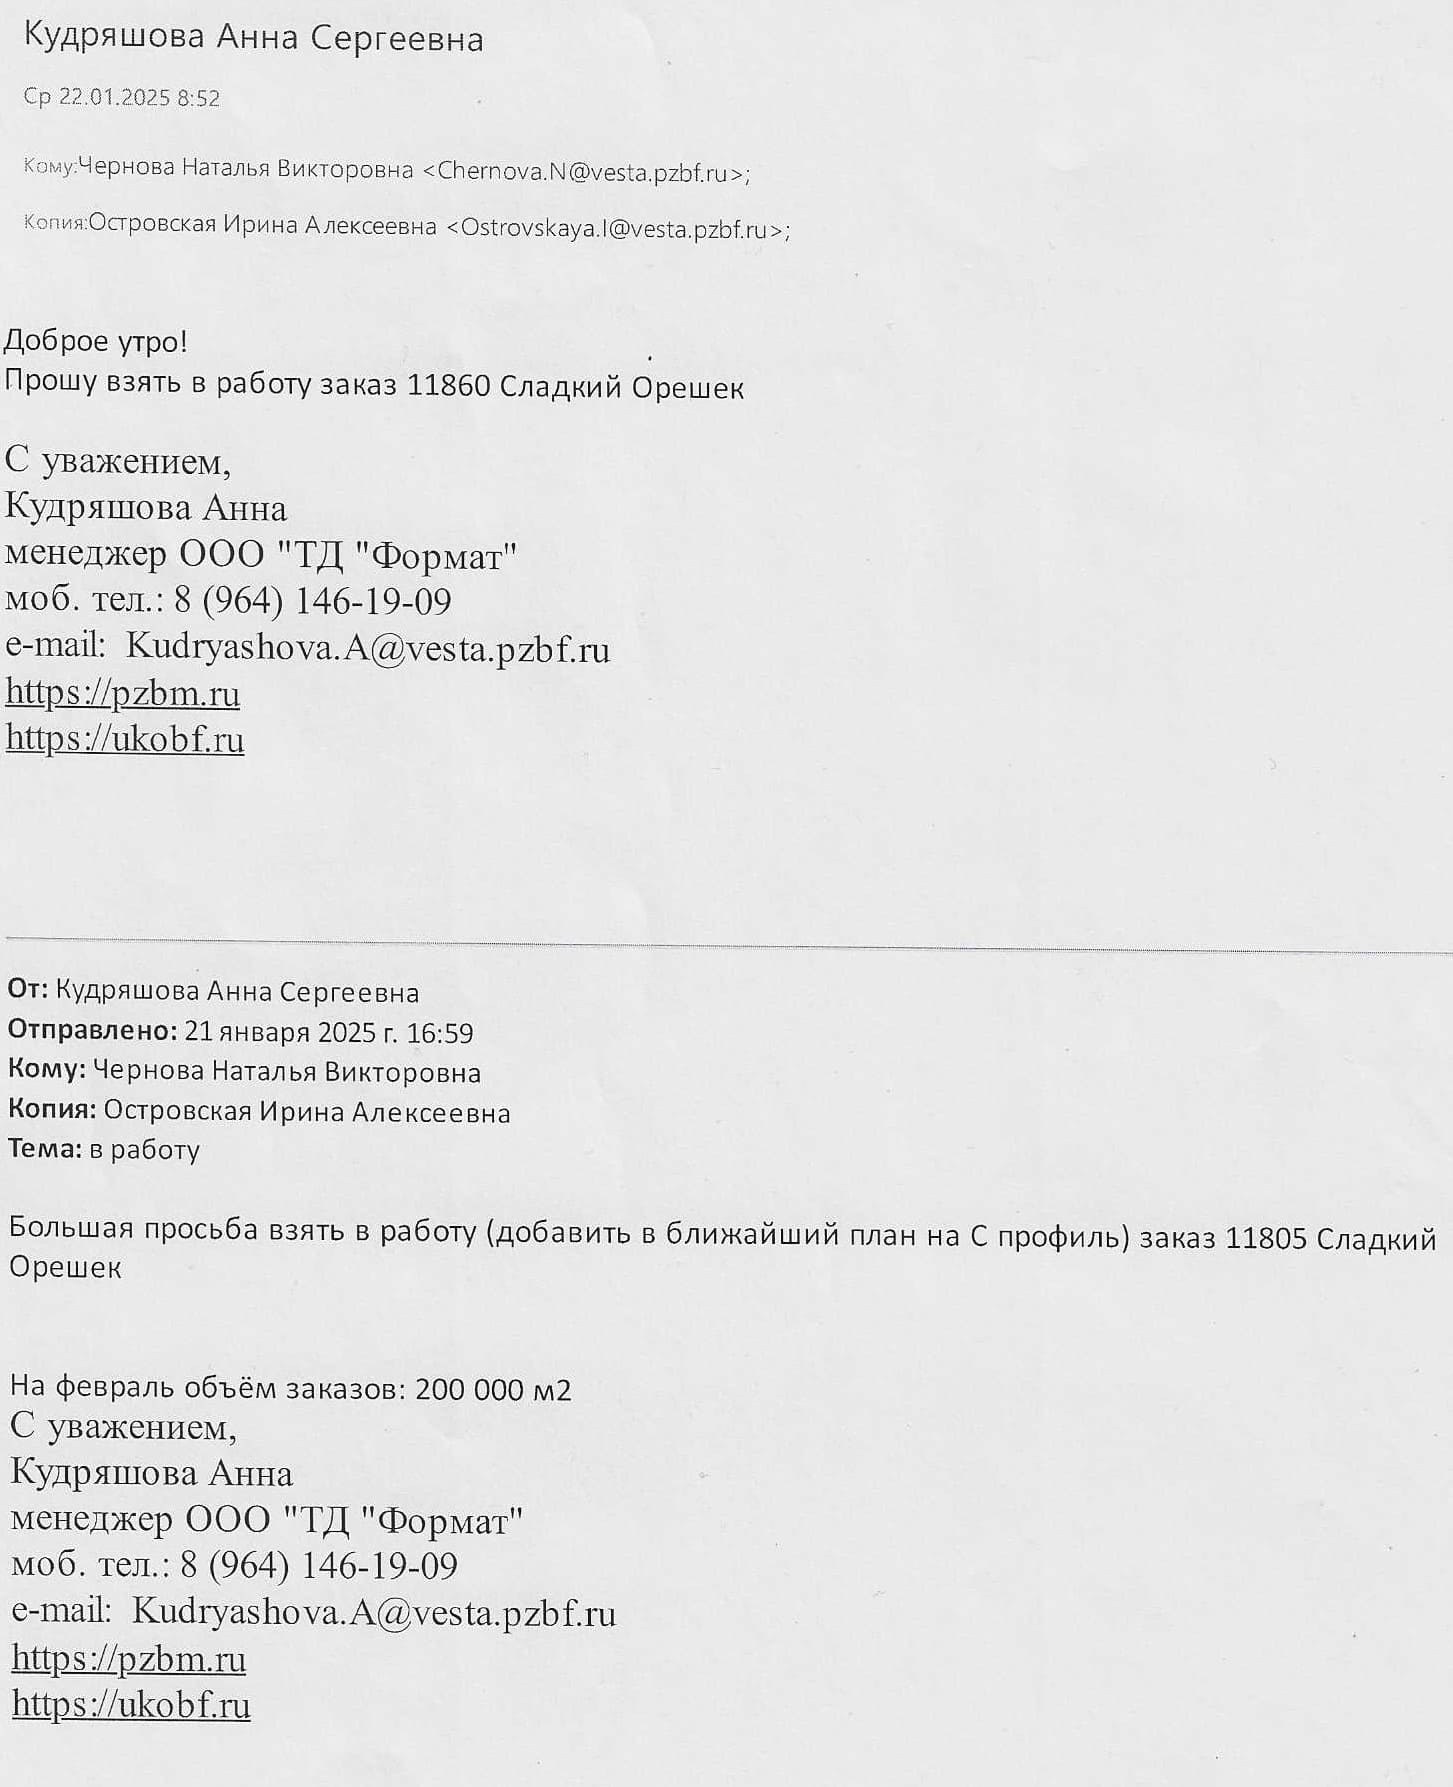
\includegraphics[height=0.7\textheight, keepaspectratio]{Pics/VII 1.jpg}
%\end{center}
%\caption{Сообщение отделу планирования о создании нового заказ}
%\label{pic:VII 1}
%\end{figure}
\clearpage

%Ежемесячно менеджеры отдела сбыта и логистики совместно с коммерческим директором разрабатывают оперативный план. 

% Разрез планирования: виды выпускаемой продукции, декада месяца.
% Показатель планирования: метры квадратные по готовой продукции.
 
%Позаказный учет отсутствует.
 
%Для каждой позиции указывается заказчик, размеры изделия, марка, оснастка, композиция сырья, план в производство и факт производства и отгрузки.

%План создается по каждому менеджеру. Оперативный план продаж является документом, по которому формируются все дальнейшие планы: план производства, план работы гофроагрегата, план работы перерабатывающих линий, план потребности в материалах, план отгрузки.
%Форма плана приведена на рис. \ref{pic:salesplan}.
%
% \begin{figure}
% \begin{center}
%  
\includegraphics[height=0.94\textheight, width=0.9\textwidth,  keepaspectratio]{Pics/Pattern.jpg}
% \end{center}
%  \caption{Форма заказа покупателя в системе СБИС}
%  \label{pic:d14}
% \end{figure}
% \clearpage


% \begin{figure}
% \begin{center}
%  \includegraphics[height=0.94\textheight, width=0.9\textwidth,  keepaspectratio]{Pics/pic.jpg}
% \end{center}
%  \caption{Цепочка заказов для планирования}
%  \label{pic:pic_d14}
% \end{figure}
% \clearpage

%
%



%Оперативное планирование определяется на основе формы \ref{pic:monthplan}, куда менеджер фиксирует все поступающие заявки.
%Производство каждый день  сообщает менеджерам коммерческого отдела  результаты работы производства. 
%При этом плановик  звонит менеджеру коммерческого отдела и говорит какие заказы приняты в производство на текущую дату.
%%Специалисты отдела планирования сообщают план выполнения на 2 дня. 
%Планировщик сообщает дату, на которую поставлен заказ. Так менеджеры узнают, когда их заявка покупателя поставлена в работу. 
%Дата (период) производства в форме плана  (см рис. \ref{pic:monthplan}) уже согласована.
%В программе 1С менеджер создает надокумент ''Счет''  и печатает форму заказа на отгрузку, в котором указывает дату отгрузки, адрес доставки, номенклатуру продукции, цены, объём. 


%\begin{figure}
%\begin{center}
%  \includegraphics[height=0.94\textheight, keepaspectratio]{Pics/prodline_loading.jpg}
%\end{center}
%  \caption{Отчет по загруженности линий}
%  \label{pic:prodline_loading}
%\end{figure}

%\clearpage
%\ifx \notincludehead\undefined
\normalsize
\end{document}
\fi